% !TeX root = 00General.tex
\thispagestyle{standard}
\pagestyle{standard}
\chapter{Ausgangslage}
\label{ausgangs}

Ein Netzwerkmanagement für ein kleines Netzwerk soll eingerichtet werden. Dafür werden die Tools Cacti und Check\_MK verwendet, die auf einer Ubuntu VM installiert werden. Die Router und Switches sollen mittels \ac{SNMP} überwacht werden. Die Server werden mittels des Check\_MK-Agents überwacht.

\chapter{Topologie und IP-Adressen}
\label{topo}

TODO: Kurz reinschreiben was welche IP hat. evtl kurze topografik


\chapter{Switch und Routerkonfiguration}

Auf den Routern und Switches wurde \ac{SNMP} konfiguriert. Der Zugriff sollte auf read-only eingestellt werden. Die Community wurde entsprechend dem zugewiesenen Städtenamen konfiguriert, in diesem Fall "innsbruck".

\section{Switch}

\lstset{escapeinside={\%*}{*)},numbers=left}%oder numbers=left
\begin{lstlisting}[caption={SNMP-Config Switch},label={lst:switch},language={}]
snmp-server community innsbruck RO
snmp-server enable traps snmp authentication linkdown linkup coldstart warmstart
snmp-server enable traps transceiver all
snmp-server enable traps call-home message-send-fail server-fail
snmp-server host 192.168.5.4 version 2c innsbruck
\end{lstlisting}

Die Traps werden an den Check\_MK server übertragen.


\section{Router}

Beim Router wurde \ac{SNMP} mitsamt allen Traps aktiviert.

\lstset{escapeinside={\%*}{*)},numbers=left}%oder numbers=left
\begin{lstlisting}[caption={SNMP-Config Router},label={lst:router},language={}]
snmp-server community innsbruck RO
snmp-server enable traps snmp authentication linkdown linkup coldstart warmstart
snmp-server enable traps vrrp
snmp-server enable traps transceiver all
...
snmp-server host 192.168.5.4 version 2c innsbruck
\end{lstlisting}

Die Konfiguration ist ähnlich wie schon beim Switch, auch hier werden die Traps an den gleichen Server übertragen.



\chapter{Cacti}
\label{cacti}

Auf dem Ubuntu-Server (IP: 192.168.5.5) wurde Cacti installiert. Die Installation gestaltet sich sehr einfach, da bereits ein Paket vorliegt. 
So genügte \texttt{apt-get install cacti} um Cacti zu installieren.

Im Webinterface wurden anschließend die beiden Netzwerkkomponenten hinzugefügt. Cacti wertet dann die \ac{SNMP}-Werte aus und kann sie grafisch darstellen.

\begin{figure}[H]
	\centering
	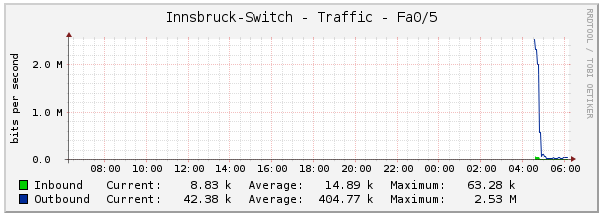
\includegraphics[width=0.9\textwidth]{img/andi_youtube.PNG}
	\caption{Netzwerkauslastung am Switch}
	\label{img:yt}
\end{figure}

In Abbildung \ref{img:yt} sieht man die Auslastung an Port 5 des Switches kurz nachdem ein Video gestreamt wurde. 

\begin{figure}[H]
	\centering
	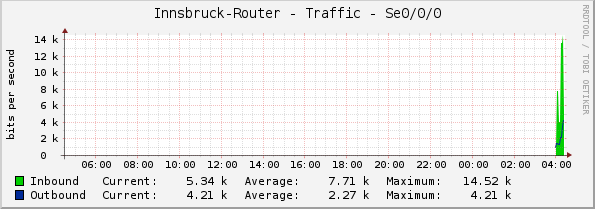
\includegraphics[width=0.9\textwidth]{img/cacti_graph_s00.PNG}
	\caption{Netzwerkauslastung am Router}
	\label{img:uplink}
\end{figure}

Auch der serielle Uplink am Router kann grafisch dargestellt werden, wie in Abbildung \ref{img:uplink} zu sehen ist.

\chapter{Check\_MK}
\label{checkmk}



\section{Switches}

Um nun die EtherChannel Technologie zu realisieren wurden die Ports "FastEthernet 23 und 24" verwendet. Diese werden als sogenannte "Trunk Links" konfiguriert.

\lstset{escapeinside={\%*}{*)},numbers=left}%oder numbers=left
\begin{lstlisting}[caption={Setting EtherChannel on a switch},label={lst:etherchannel},language={}]
interface FastEthernet0/24
 switchport trunk allowed vlan 10,20,30
 switchport mode trunk
 channel-protocol lacp
 channel-group 1 mode active
\end{lstlisting}

Des weiteren wurden die verschiedenen \ac{VLAN}s, die auf den jeweiligen Switches hängen, eingestellt.

\lstset{escapeinside={\%*}{*)},numbers=left}%oder numbers=left
\begin{lstlisting}[caption={VLAN Konfiguration auf Switch 1},label={lst:vlan},language={}]
interface Vlan10
 ip address 192.168.5.254 255.255.255.0
!
interface Vlan20
 ip address 192.168.15.254 255.255.255.0

\end{lstlisting}

\section{Router}

Als internes Routing Protokoll wurde \ac{OSPF} verwendet. Um \ac{OSPF} richtig zu konfigurieren muss jedem Router eine eindeutige "router-id" zugewiesen werden, sowie alle bekannten Netze in der entsprechenden Area eingetragen werden.

\lstset{escapeinside={\%*}{*)},numbers=left}%oder numbers=left
\begin{lstlisting}[caption={OSPF Konfiguration auf Router 1},label={lst:ospf},language={}]
router ospf 10
 router-id 1.1.1.1
 network 10.10.10.0 0.0.0.255 area 0
 network 172.16.5.0 0.0.0.3 area 0
 network 192.168.5.0 0.0.0.255 area 0
 network 192.168.15.0 0.0.0.255 area 0


\end{lstlisting}